  \section{System Design and Architecture}
  \label{sec:system-design}

  In this chapter, the architecture of the system is described. The system is designed to achieve following goals. The system should be modular and easily extensible to allow future extensions towards a full model transformation platform for production use cases. The system should also be maintainable. In the folowing sections, the high-level architecture following the \ac{glsp} architecture is described. Then the design of the components, control flow and data models is described. In the end the UI design is explained.

  \subsection{Design Decisions}
  \label{subsec:design-decisions}

  In the section \ref{sec:background} the used frameworks and technologies were described. The selection of these framworks still leave some open design decisions. One open decision was which platform integration to use for the \ac{glsp} client. \ac{glsp} can be used as an extension for Eclipse Theia or \ac{vscode}, a plugin for the Eclipse \acs{ide} or as a standalone web application. They can also be used in combination, but to avoid overhead and complexity, only one platform integration is initially used. In table \ref{tab:glsp-platform-comparison} the different integration options are compared. Since the integration into an existing \acs{ide} fits the graph editors, the standalone editor is not an option. For that, many additional features like a file explorer have to be implemented. The integration into the Eclipse \acs{ide} is also not an option, since it is not based on web technologies and therefore not satisfying the requirements of the project. Between the Eclipse Theia and \ac{vscode} integration, Eclipse Theia is providing more flexiblity in the usage and deployment of the application. Next to the usage as an extension that can be added during runtime, Theia also provides the option to bundle your own \ac{ide} including the \ac{glsp} graph editors. That makes it deployable as a complete application, where no additional plugins are needed. This flexibility is the main reason to choose the Eclipse Theia integration as the inital main platform for Henshin Web. With that usage and deployment flexibility, different additional platform integrations are probably not needed in the future.

  \begin{table*}[h]
    \centering
    \caption{Comparison of GLSP Platform Integrations}
    \label{tab:glsp-platform-comparison}
    \resizebox{\textwidth}{!}{
        \begin{tabular}{|p{3cm}|p{3cm}|p{3cm}|p{3cm}|p{3cm}|}
            \hline
            \textbf{Criteria} & \textbf{Eclipse Theia} & \textbf{\ac{vscode}} & \textbf{Eclipse \acs{ide}} & \textbf{Standalone} \\
            \hline

            \textbf{Deployment Options} & Web-app, Desktop (Electron) & Desktop, Web-app & Desktop & Custom (Web or Desktop)\\
            \hline
            \textbf{Extendability} & Access to all Theia internal \acsp{api} & Through VS Code Extension \acsp{api} & Moderate, via Eclipse plugins (OSGi-based) & Fully customizable (with own implementations) \\
            \hline
            \textbf{Provided Environment} & Complete \acs{ide} & Complete \acs{ide} & Complete \acs{ide} & No other features included \\
            \hline
            \textbf{Result Format} & Own \acs{ide} or as a plugin & \ac{vscode} extension & Eclipse \acs{ide} plugin & javascript based web editor module \\
            \hline
            \textbf{Dependencies Needed} & browser & \ac{vscode} Desktop or browser & Eclipse \acs{ide}& browser \\
            \hline
        \end{tabular}
    }
\end{table*}



  Another decision was to select a edge routing style. \ac{glsp} provides two different routing algorithms, the Manhattan and Polylime stlyes. The Manhattan style was invented by \citeauthor{manhattan} to achieve wire length optimization in circuit design.  It only uses vertical and horizontal lines to connect nodes. \cite{manhattan}. The conncetion can be split into multiple segments, changing from a horizontal to a vertical line or the other way round to create a stair like connection between nodes. The Polyline style on the other hand uses straight lines to connect nodes. They line can also be split into multiple segments with arbitrary angles between them.
  For this use case, the main aspect is the clarity and readability of the graph. You can see the comparison of the two styles in figure \ref{fig:edge-kind-comparison}. Advantages of the Manhattan style are that can prevent edge crossings, and therefore can help reduce visual clutter. In complex diagrams with many nodes and edges, it is easier to trace the horizontal and vertical lines. On the other hand, it can overlap with other edges, which can make it hard to follow the edge. Especially named edges that overlaps partly with another edge can't be followed without clicking and highlighting it. You can see that in figure \ref{fig:edge-kind-comparison} between the \textit{Bank-Account} and the \textit{Account-Client} edge. To prevent that, the edge routing needs be stored in the notation file to be able to persist changes in the routing that remove overlapping edges. The Polyline style on the other hand is generally simpler and more compact. It can get very clutterd with many edges crossing and other nodes overlapping the diagonal lines. Metamodel, transformation rules and instances are typically not that complex, so that a simple line bewteen nodes is sufficient and additonal edge segments are not needed. Because of that, the edge placement doens't have to be stored in the notation file. The edge automatically aligns itself when a node is moved. The rotation of the edge label that it runs parallel with the line supports the simple and compact design of the Polyline style. To additionally prevent crossing lines, a option to dynammically hide the root node and its edges in \ac{xmi} graphs is introduced.

  \begin{figure}
    \centering
    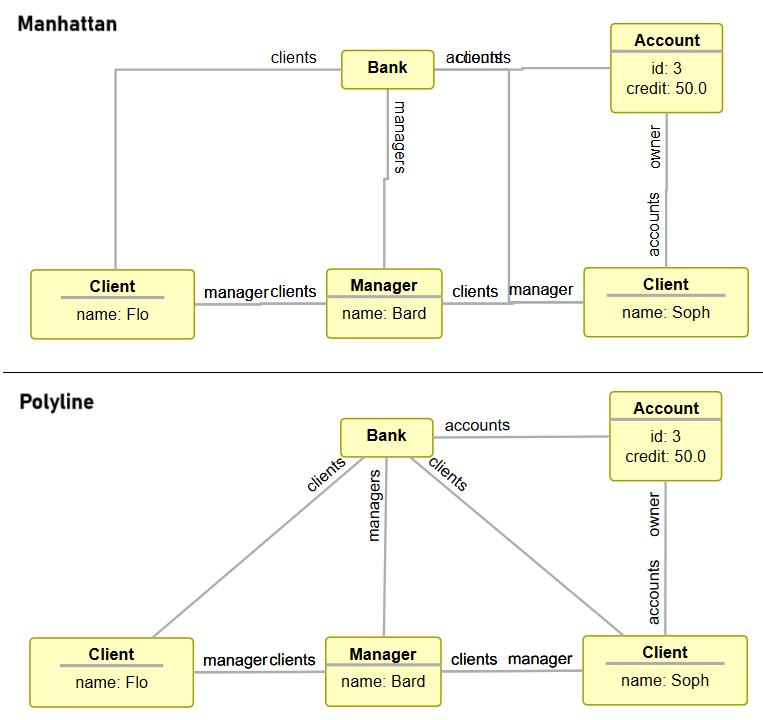
\includegraphics[width=0.7\textwidth]{edge-kind-comparison}
    \caption{Visual comparison of the two edge routing styles of \ac{glsp}}
    \label{fig:edge-kind-comparison}
  \end{figure}

    One main question in the UI design was where to put the selection of the transformation rules of a \textit{.henshin} file. There are several options to display the rule seletion. The first option is to add the list of rules to the tool palette as an additional pallete group next to the nodes and edges. Here no additional new UI element must be placed in the graph editor, but the main focus of the tool palette is to provide editing tools of the graph elements. Swapping between the rules doesn't fit into the main purpose of the tool. Another option is to create a custom UI element that is displayed in the rule graph editor. I would be easy to implement, directly integrated into the graph module and platform independent. But it would take up additional space in the graph editor view. The rule graph should be the main focus of the application and should have enough space to display the graph elements, especially for larger graphs.

    For these two options, the user also has always to switch to the rule graph editor first to select a rule. It can negatively impace toe user experience. That would not be the case if the rule selection is integrated into the Theia explorer. Since the custom explorer is used anyway to select between different instance, transformation rule or metamodel files, it is a good place to also select the transformation rules. The explorer can also be collapsed to save more space for the graphs and for very many rules it automatically supports scrolling. Extending theia internal \acs{api} makes it more effort to add aditional \ac{glsp} platform integrations, because the custom changes need to be newly implemented for the new platform, it may even not support the same extendability. Since the theia integraion provides the most options to use and deploy the application, more platform integrations are probably not needed. Aditionally, the extension of the theia explorer prevents the occupation of additional space in the \ac{glsp} editor widget to select a rule. This improvement of the user experience and intuitiveness outweights the possible additional effort for new platform integrations. The implementaiton of the custom explorer is described in section \ref{subsec:custom-ui-extensions}.


  \subsection{Following the \ac{glsp} Architecture}
  \label{subsec:high-level-architecture}

  The system is based on the \ac{glsp} architecture, that uses a client-server architecture. The client and server communicate via a websocket connection and JSON-RCP. The \ac{glsp} server can be implemented with Java or Node.js, but due to the constraint that Henshin is implemented in Java, the server is also implemented in Java. The client is implemented in TypeScript. \ac{glsp} provides a defined protocol for the communication between client and server, which can extended with custom commands and actions. The communication is performed using Action Messages, that can be sent from the client and the server to each other or also to itself. The client and the server have Action Handlers, that process the Action Messages and perform the corresponding actions. Each client connection starts its own server instance, therefore each server is only responsible for one client. \cite{glsp-doc} Since each client needs to be able to display three different graph editors for different file types, the server consists of three diagram modules. Each diagram module defines a different diagram language. The \code{XMIDiagramModule} is responsible for the editor of \ac{xmi} instance files, the \code{RuleDiagramModule} is responsible for the editor of Henshin rule files and the \code{EcoreDiagramModule} is responsible for the editor of Ecore metamodel files. In figure \ref{fig:architecture} you can see the high-level architecture of a server and client instance. The architecture of the three diagram modules is quite similar. Each diagram module has a \code{ModelState} which is the central statefull object within a client session \cite{glsp-doc}. The \code{ModelState} is accesed by all other services and handler and represents the current state of the actual source model. \ac{glsp} supports the integration of \ac{emf} models as the underlying source model for the diagrams by default. For that The \code{EMFSourceModelStorage} can load a \ac{emf} file as a \code{RessourceSet}, that is then attached to the \code{ModelState}. That allows an simple integration of the Henshin SDK, since it based on \ac{emf} and provides a \code{HenshinRessourceSet} can be loaded directly over the \ac{emf} integration of \ac{glsp} into the \code{ModelState}.

  The \code{ModelState} of each diagram module also contains an index and a notation model for the layout of the elements in the graphical editor. To be able to have a consistent layout of the elements, not changing after every reload or action, the position and size of each element for each model file is stored in a seperate \textit{.notation} file. The index of the \code{ModelState} is used to map the elements of the source model to the graphical model of \ac{glsp}. For each diagram module, the indexing is implemented in a different way. (see section \ref{subsec:indexing} for more details).

  Another important part of each diagram module is the \code{GModelFactory}, which is responsible for creating the graphical model that is sent to the client from the source model. Since metamodel, transformation and instance \ac{emf} model are strucutred differently, each \code{GModelFactory} of each diagram module is implementing its own mappings.

  \begin{figure}
    \centering
    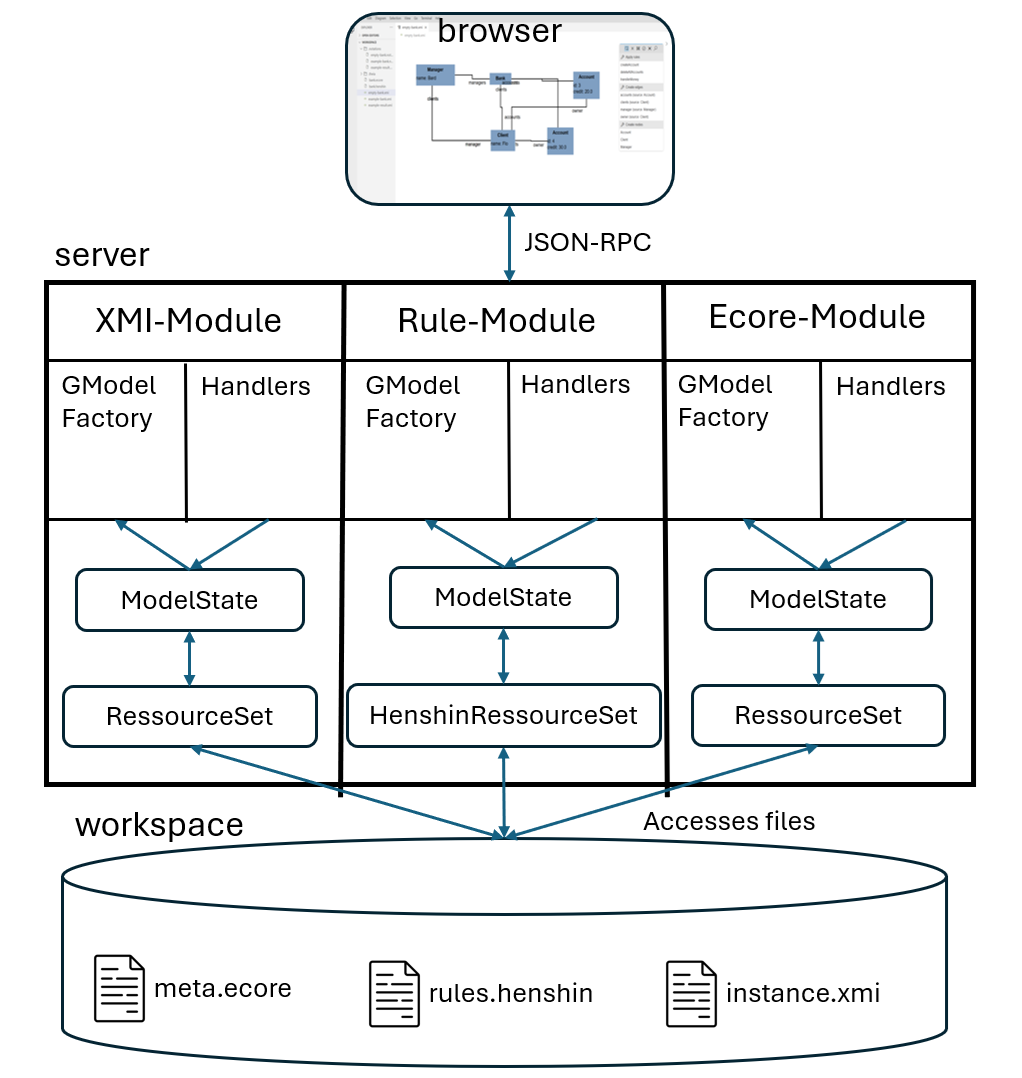
\includegraphics[width=0.6\textwidth]{architecture.png}
    \caption{High-Level Architecture of the System}
    \label{fig:architecture}
  \end{figure}

  \subsection{Data Models and Structures}
  \label{subsec:data-models}

  All three diagram modules have an \ac{emf} based source model. For the Ecore metamodel and the \ac{xmi} instances, The standard data model of \ac{emf} is used. As described in section \ref{subsec:emf} different implementations of \code{EObject} are used, representing all used elements like nodes, attribues or references. For the Hensin transfomations model, the data model of the Henshin \ac{sdk}, that builds upon the \ac{emf} data model, are used. No additional data structures are needed, since every created domain model is based on the \ac{emf} data model. The data model of the graphical representation is provided by \ac{glsp}. It can be extended with custom elements, but the default elements are sufficient for the current use cases. 

  The user has to select or create a workspace in the UI, where all the source models are located. Each workspace for Henshin Web has to be in a specific structure. It should contain one \textit{.ecore} metamodel and one \textit{.henshin} transformations file. Additionally, arbitrary \textit{.xmi} instance files can be added. All of these files should be stored in the root folder of the workspace. When creating a new model file or opening it for the first time, a new notation file is generated and stored in the \textit{.notation} subfolder of the workspace. These notation files are not displayed in the theia explorer.  

  \subsection{\ac{glsp} Client Structure}
  \label{subsec:component-design}

  The \ac{glsp} client is divided in different main modules.
  The \textit{henshin-glsp} module is responsible for platform independent code. It contains client side action handlers, custom UI extensions and custom graph elements. This module is used by the three theia specific modules, that are responsible for the integration of the \ac{glsp} client into the Eclipse Theia framework. There is one module for each diagram type. The target specific code is loacted here. One example is the customization of the Theia explorer view, that it also displays all rules of a \textit{.henshin} file and hides the notation files. These three theia extensions are then combined in the \textit{henshin-browser-app} module, that has no additional code, but only combines the three theia modules into one application. 

  \subsection{User Interface Design}
  \label{subsec:user-interface-design}

  The design of the user interface is based on the design principles of \ac{glsp} and Eclipse Theia. For editing the graphs, the main UI element is the tool palette on the right side of the graph editor. It lists all available nodes and edges, that can be added to the graph as well as the transformation rules that can be applied. It also contains a set of predefined \ac{glsp} actions, which are switching between selection mode, deletion mode and marquee mode, as well asreseting the viewport and search for tool palette entries. For keyboard usage, ther is also the command palette, that can be opened with the \textins{Ctrl + Space} shortcut. It opens a searchbar with a list of options below. Here all editing operations are registered listed and can be performed by searching or navigating through the list and selecting the desired operation. 
  
  The design of the custom UI elements like the parameter selection form or the display of the transformation rule information follows the design of \ac{glsp}. The design of Theia uses a flat design with minimal gradients, shadwos or 3D elements. Compared to that uses \ac{glsp} a more 3D-like design with shadows and gradients, because the UI elements need to be on top of the main graph plane. That shows that the UI elements are not part of the graph, but are additoinal elements to interact. The tool palette, comamnd pallete and context menu all use shadows and rounded eges. New custom UI elements like the parameter selection also use the same shadow and rounded corners to also show that they are not part of the graph, but elements to interact with.

  The colors of the custom UI elements follows the color theme of Theia. Important is that Theia uses the dark mode as a default theme. Graph editors typically use a light backgroung. All custom UI elements are designed to adjust to the dark mode and use the according colors as the default dark Theia elements. The final UI can be seen in appendix \ref{fig:ecore-ui}, \ref{fig:rule-ui} and \ref{fig:xmi-ui}.

